%% ****** Start of file apstemplate.tex ****** %
%%
%%
%%   This file is part of the APS files in the REVTeX 4.2 distribution.
%%   Version 4.2a of REVTeX, January, 2015
%%
%%
%%   Copyright (c) 2015 The American Physical Society.
%%
%%   See the REVTeX 4 README file for restrictions and more information.
%%
%
% This is a template for producing manuscripts for use with REVTEX 4.2
% Copy this file to another name and then work on that file.
% That way, you always have this original template file to use.
%
% Group addresses by affiliation; use superscriptaddress for long
% author lists, or if there are many overlapping affiliations.
% For Phys. Rev. appearance, change preprint to twocolumn.
% Choose pra, prb, prc, prd, pre, prl, prstab, prstper, or rmp for journal
%  Add 'draft' option to mark overfull boxes with black boxes
%  Add 'showkeys' option to make keywords appear
\documentclass[aps,preprint,amsmath, amssymb]{revtex4-2}
%\documentclass[aps,prl,preprint,superscriptaddress]{revtex4-2}
%\documentclass[aps,prl,reprint,groupedaddress]{revtex4-2}
\usepackage{hyperref}
\usepackage{graphicx}% Include figure files
\usepackage{dcolumn}% Align table columns on decimal point
\usepackage{bm}% bold math
\usepackage{braket}


% You should use BibTeX and apsrev.bst for references
% Choosing a journal automatically selects the correct APS
% BibTeX style file (bst file), so only uncomment the line
% below if necessary.
%\bibliographystyle{apsrev4-2}

\begin{document}

% Use the \preprint command to place your local institutional report
% number in the upper righthand corner of the title page in preprint mode.
% Multiple \preprint commands are allowed.
% Use the 'preprintnumbers' class option to override journal defaults
% to display numbers if necessary
%\preprint{}

%Title of paper
\title{Microscopic ensemble bootstrap in phase space}

% repeat the \author .. \affiliation  etc. as needed
% \email, \thanks, \homepage, \altaffiliation all apply to the current
% author. Explanatory text should go in the []'s, actual e-mail
% address or url should go in the {}'s for \email and \homepage.
% Please use the appropriate macro foreach each type of information

% \affiliation command applies to all authors since the last
% \affiliation command. The \affiliation command should follow the
% other information
% \affiliation can be followed by \email, \homepage, \thanks as well.
\author{y}
%\email[]{Your e-mail address}
%\homepage[]{Your web page}
%\thanks{}
%\altaffiliation{}
\affiliation{hhu}

%Collaboration name if desired (requires use of superscriptaddress
%option in \documentclass). \noaffiliation is required (may also be
%used with the \author command).
%\collaboration can be followed by \email, \homepage, \thanks as well.
%\collaboration{}
%\noaffiliation

\date{\today}

\begin{abstract}
% insert abstract here
    The bootstrap method which has been studied under many quantum mechanical models turns out to be feasible in microcanonical ensemble as well. In this paper we report a method as a improvement to [Y.\ Nakayama, Modern\ Physics\ Letters\ A\ \textbf{37}, 10.1142/s0217732322500547 (2022)].
\end{abstract}

% insert suggested keywords - APS authors don't need to do this
%\keywords{}

%\maketitle must follow title, authors, abstract, and keywords
\maketitle

% body of paper here - Use proper section commands
% References should be done using the \cite, \ref, and \label commands
\section{Introduction}
% Put \label in argument of \section for cross-referencing
%\section{\label{}}
The bootstrap method aims at solving a system with its fundamental constraints, the so called positivity constraints. Although widely used in quantum mechanics, one can also apply the method into microcanonical ensembles which can be seen as classical correspondence to the quantum mechanical case when $\hbar \to 0$. Nakayama first introduced this method into the classical scenario~\cite{Nakayama_2022}, but he mentioned a peninsula in $ E < 0$ which doesn't converge even for stronger constraints. In our work, we use both position $x$ and momentum $p$ in the phase space to bootstrap, we can see the peninsula shrinks vastly compared to the $x$ only bootstrap program.

\section{Bootstrapping Method}
\subsection{Bootstrap Equations and Matrices}
Starting with the Hamiltonian we have
\begin{equation}
    H = \frac{p^2}{2M} + V(x)
\end{equation}
for microcanonical ensemble the average of an observable $\mathcal{O}(x, p)$ is
\begin{equation}
    \braket{\mathcal{O}(x, p)} = \frac{\int dxdp\mathcal{O}(x, p)\delta (E - H)}{\int dxdp\delta (E - H)}
\end{equation}
and we can easily find that
\begin{align}
    \braket{\{H, \mathcal{O}\}} = 0 \label{eq:beq0}\\
    \braket{H \mathcal{O}} = E \braket{\mathcal{O}} \label{eq:beq1}
\end{align}
here $\{H, \mathcal{O}\}$ is the poisson bracket.
As for the positivity constraints, obviously that for any observable $\mathcal{O}$ we would have
\begin{equation}
    \braket{\mathcal{O}^* \mathcal{O}} \geq 0
\end{equation}
and by writing the observale as a polynomial of certain observable $o$, $\mathcal{O} = \sum_{i = 0}^k a_i o^i$, one can construct a bootstrap matrix which can be defined as
\begin{equation}
    \bm{\mathcal{M}}_{ij} = \braket{(o^*)^i o^j}, \ \ \ i, j = 0, 1, ..., k
\end{equation}
we can then rewrite the constraints (5) with matrix and vectors
\begin{equation}
    \bm{\alpha}^\dagger \bm{\mathcal{M} \bm{\alpha}} \geq 0\label{eq:positivity}
\end{equation}
as ~\eqref{eq:positivity} should hold true for any vector $\bm{\alpha}$, the bootstrap matrix $\bm{\mathcal{M}}$ must embody the positive semi definiteness i.e. $\bm{\mathcal{M}} \succeq 0$, which is essentially an eigenvalue problem
\begin{equation}
    \forall (\bm{\mathcal{M}})_{eigenvalue} \geq 0
\end{equation}
When the observable $\mathcal{O}$ is a coupling of two observables, say, $A$ and $B$
\begin{equation}
    \mathcal{O} = \sum_{i, j = 0}^{k - 1} a_i b_j A^i B^j\\
\end{equation}
\begin{equation}
    \mathcal{O}^* \mathcal{O} = \sum_{i_1, j_1, i_2, j_2 = 0}^{k - 1} a_{i_1}^* b_{j_1}^* (B^*)^{j_1} (A^*)^{i_1} A^{i_2} B^{j_2} a_{i_2} b_{j_2}
\end{equation}
here we define two auxiliary matrices $\bm{\mathcal{M}}_{ij}^0 = (B^*)^j (A^*)^i$ and $\bm{\mathcal{M}}_{ij}^1 = A^i B^j$, the constraints may be written as
\begin{equation}
    \bm{\mathcal{M}}_{ij} = \braket{(\bm{\mathcal{M}}^0 \otimes \bm{\mathcal{M}}^1)_{ij}}, \ \ i, j = 0, 1, 2, ..., k^2 - 1
\end{equation}
\begin{equation}
    \bm{\mathcal{M}} \succeq 0
\end{equation}


\subsection{Double Well Potential}
The Hamiltonian of a double well potential can be written as
\begin{equation}
    H = p^2 - x^2 + x^4
\end{equation}
here we consider the observable $\mathcal{O} = x^m p^n$, substitute it as well as the Hamiltonian into \eqref{eq:beq0} and \eqref{eq:beq1}, we can obtain two recursion formulas
\begin{equation}
    2(2n + m)\braket{x^{m + 3} p^{n - 1}} = 2(m + n)\braket{x^{m + 1} p^{n - 1}} + 2mE\braket{x^{m - 1} p^{n - 1}} \label{eq:recur0}
\end{equation}
%\begin{align}
%    2(2n + m)\braket{x^{m + 3} p^{n - 1}} =& \notag \\ &2(m + n)\braket{x^{m + 1} p^{n - 1}}\notag \\ &+ 2mE\braket{x^{m - 1} p^{n - 1}} \label{eq:recur0}
%\end{align}
%\begin{align}
%    \braket{Hx^m p^n} = E\braket{x^m p^n} =&\notag \\ &\braket{x^m p^{n + 2}} - \braket{x^{m + 2} p^n}\notag \\ &+ \braket{x^{m + 4} p^n} \label{eq:recur1}
%\end{align}
\begin{equation}
    \braket{Hx^m p^n} = E\braket{x^m p^n} = \braket{x^m p^{n + 2}} - \braket{x^{m + 2} p^n}\notag + \braket{x^{m + 4} p^n} \label{eq:recur1}
\end{equation}
plus $\braket{\{H, x^m\}} = 0$, we get
\begin{equation}
    \braket{x^{m - 1} p} = 0 \label{eq:recur2}
\end{equation}
and for simplicity, we here assume that the average of $x$ to the odd powers is $0$ 
\begin{equation}
    \braket{x^m} = 0,\ \ \ \text{for all odd}\ m \label{eq:recur3}
\end{equation}
with \eqref{eq:recur0}~\eqref{eq:recur1}~\eqref{eq:recur2}~\eqref{eq:recur3} plus the initial paratemers $E$ and $\braket{x^2}$ we can construct the bootstrap matrix $\bm{\mathcal{M}}$.The result when $k = 5$ is shown in Fig.~\ref{fig:doublewell}. We also reproduced the result in \cite{Nakayama_2022} to make a comparison.

\begin{figure}
    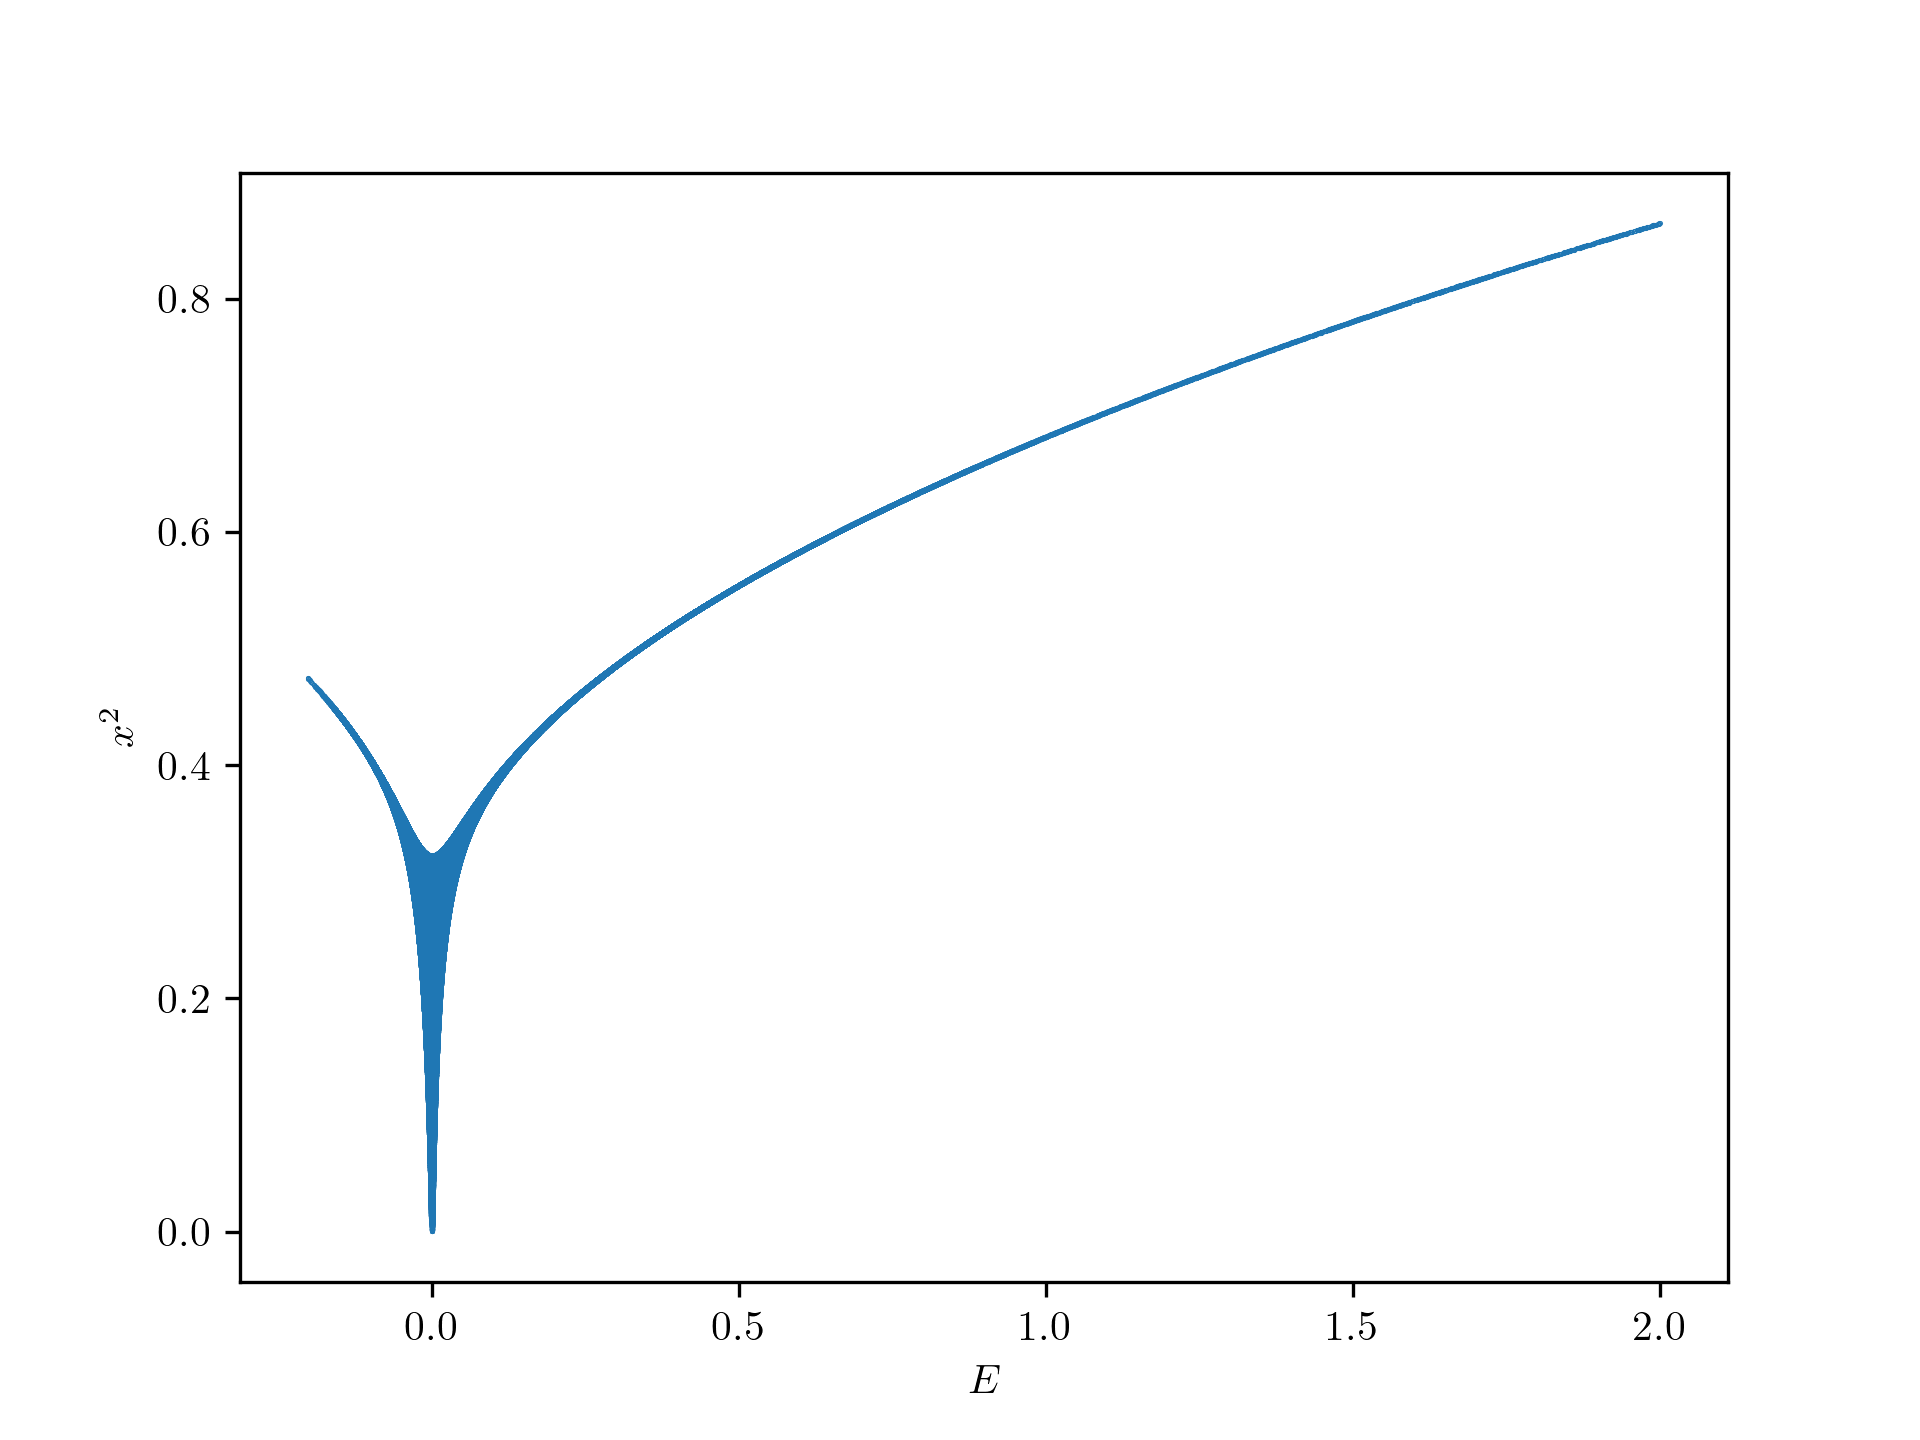
\includegraphics[width=0.45\linewidth]{plot_5.png}
    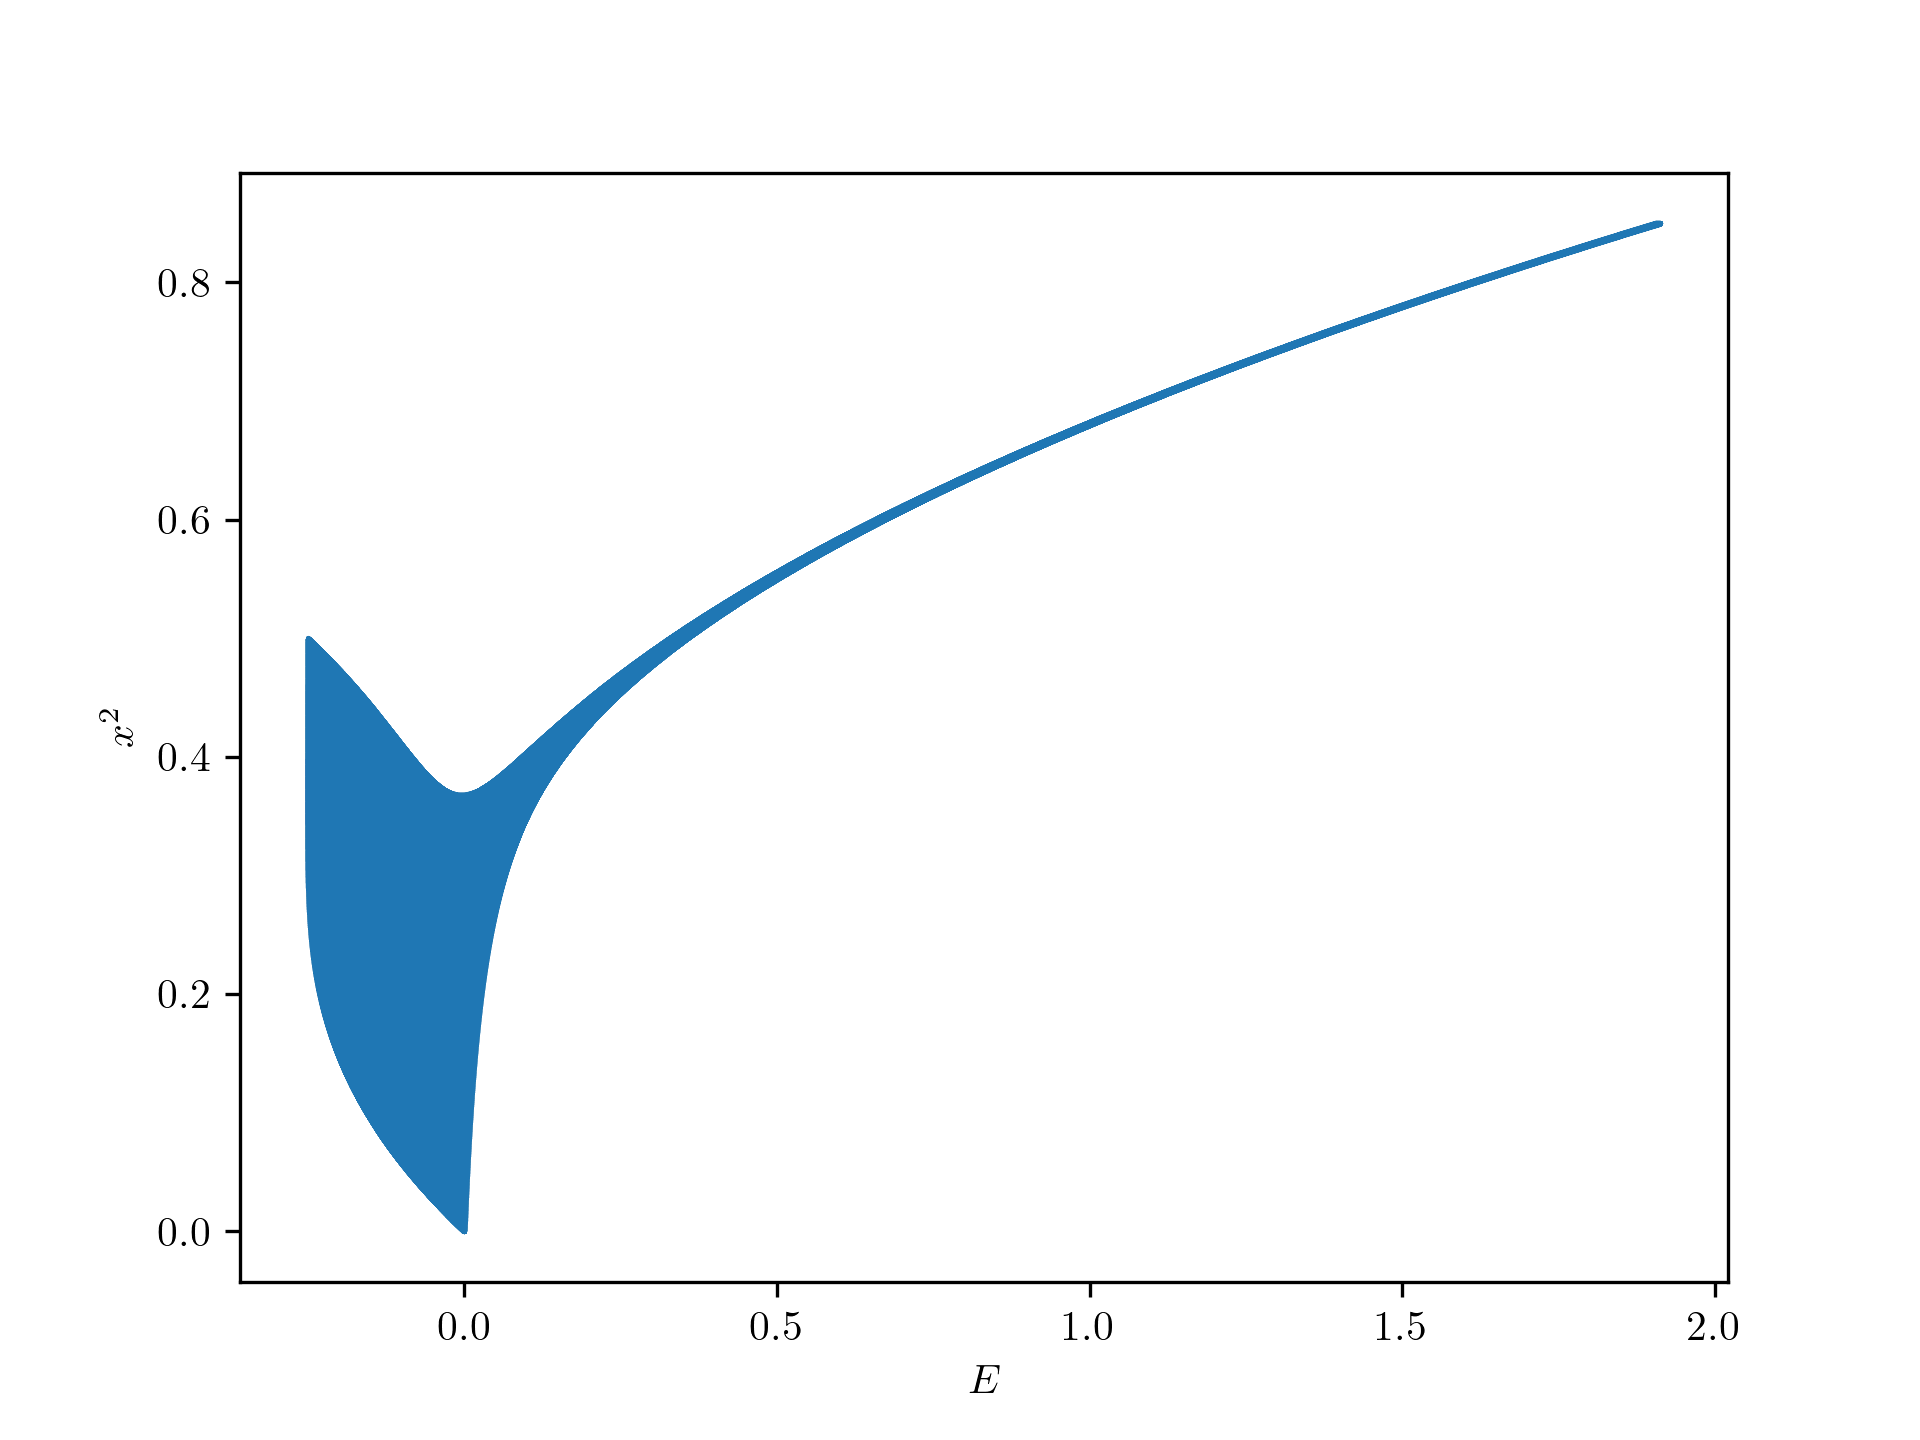
\includegraphics[width=0.45\linewidth]{x_9.png}
    \caption{$xp$ bootstrap with $k = 5$(left), $x$ only bootstrap with $k = 9$(right)}
    \label{fig:doublewell}
\end{figure}

\begin{figure}
    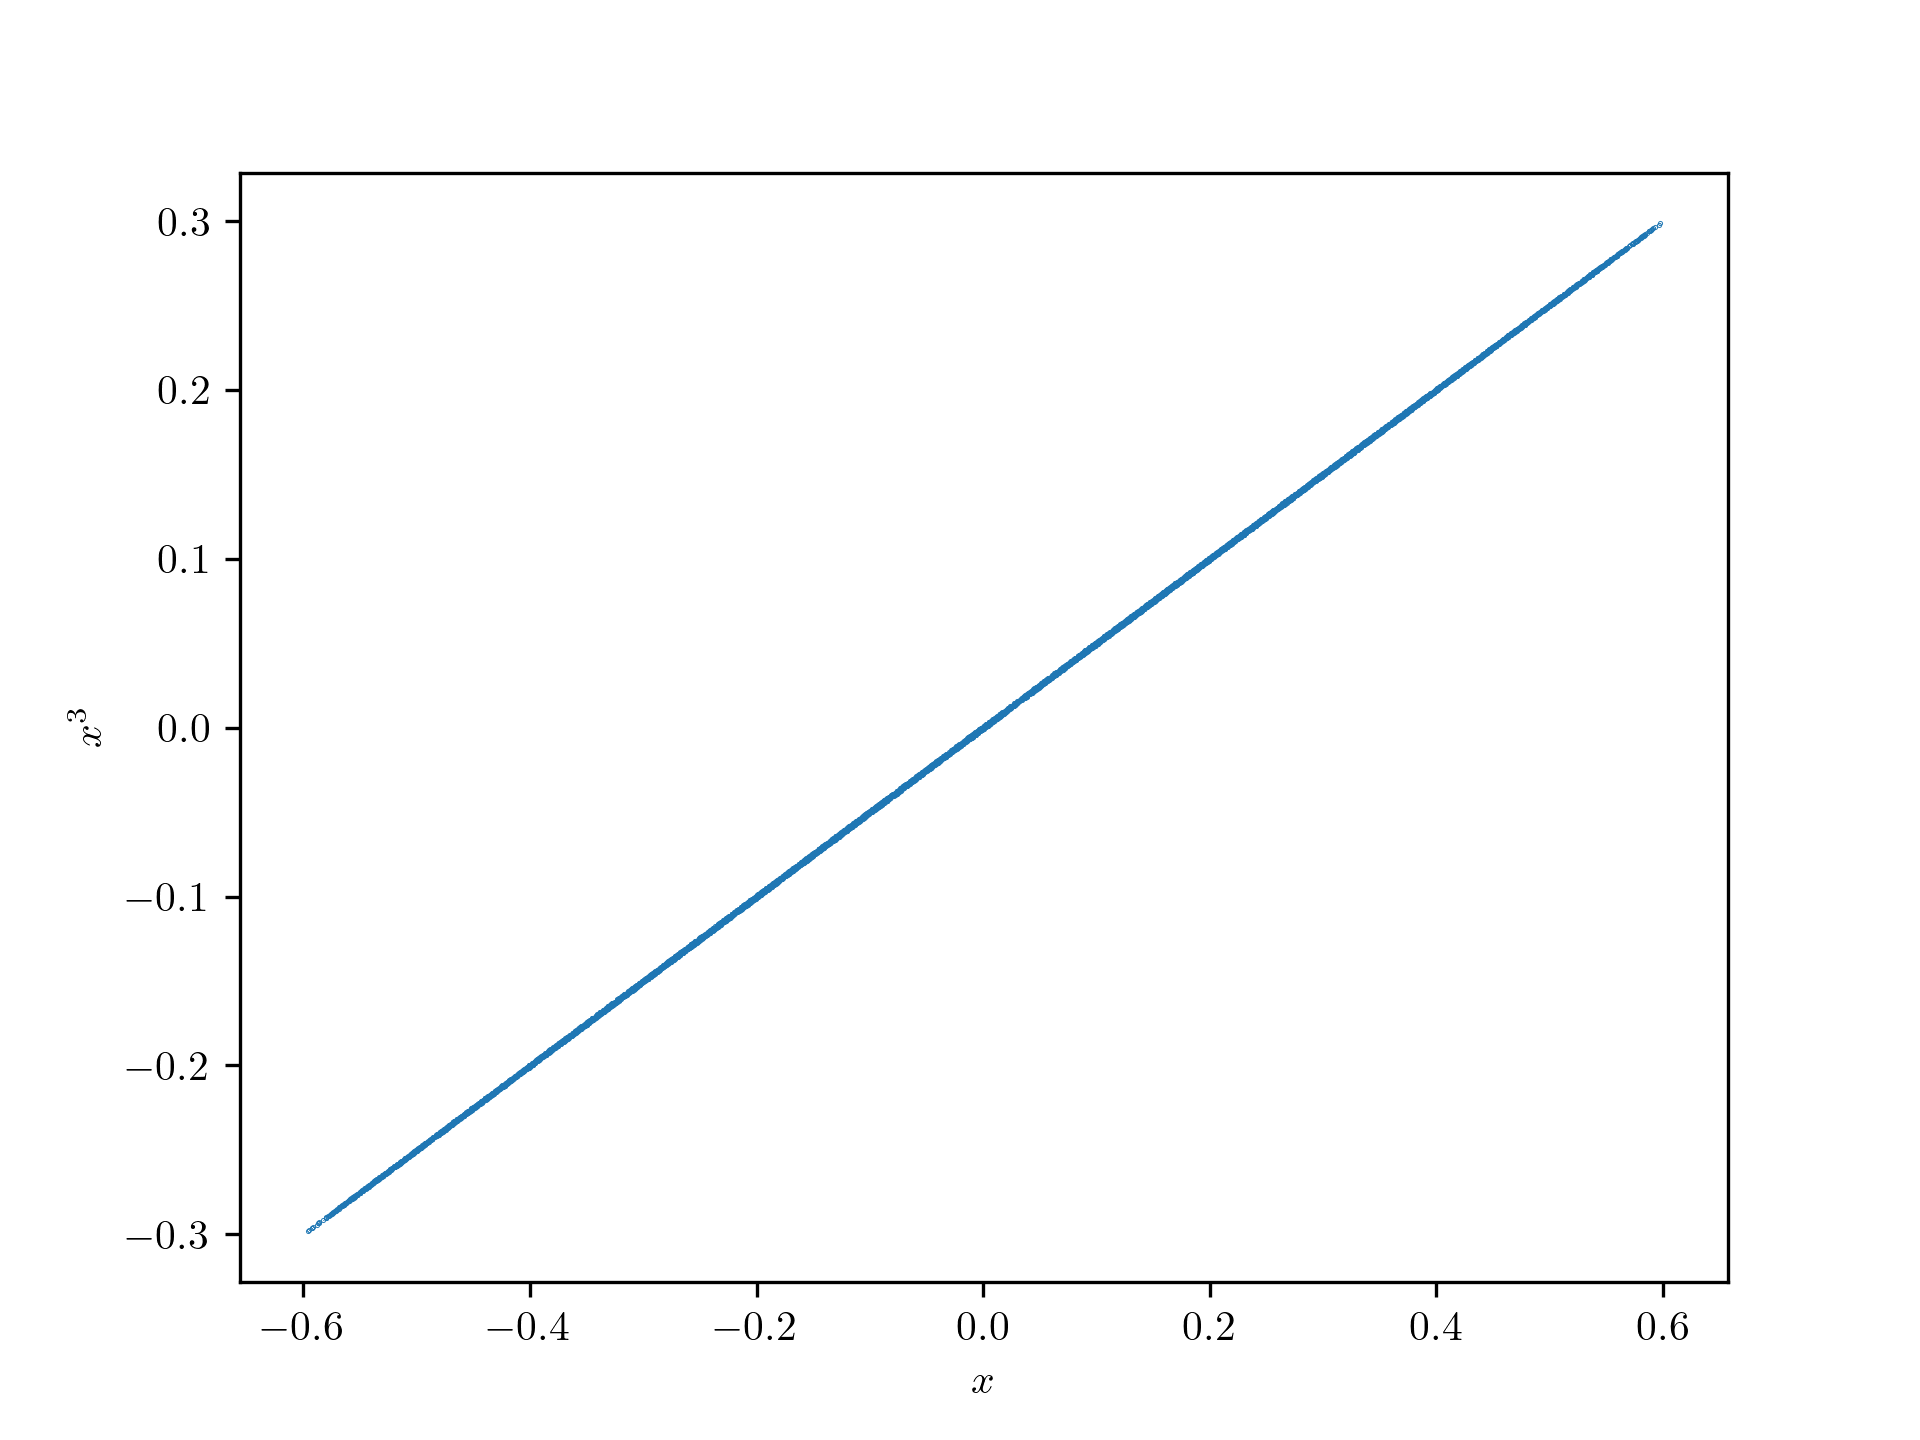
\includegraphics[width=0.8\linewidth]{13.png}
    \caption{$\braket{x^m p^n}$ bootstrap ($k = 5$) with fixed $E = -0.1$ and $\braket{x} = 0.4052$}
    \label{fig:xx}
\end{figure}


In constrast with \cite{Nakayama_2022}, our result shows no peninsula in where $E < 0$, as we include the information of the momentum. When E turns negative, the curve menifests a similar behavior as the positive part. In our program the scale of the bootstrap matrix is $k^4$, which is much larger compared to the single observable bootstrap program with the scale of $k^2$. So here the size of our bootstrap matrix is $625$, about seven times to the $x$ bootstrap. But the region still doesn't shrink even when we set $k = 25$ for the $x$ only bootstrap program, so we conclude that this bootstrap in phase space does have a much stronger constraints than the single observable one.

Like Nakayama has mentioned, $\braket{x}$ doesn't have to be zero in classical mechanics, but this method does produce a narrow region upon the assumption \eqref{eq:recur3}. So we then study the $\braket{x}$ and $\braket{x^3}$ with fixed $E$ and $\braket{x^2}$ using the $\braket{x^m p^n}$ bootstrap program, which, still turns out to be a line in Fig.~\ref{fig:xx}.

\section*{Acknowledgements}
I would like to express my sincere gratitude to my tutor, [Dong Bai], for providing valuable guidance and direction throughout the course of this research. His insights and expertise significantly contributed to the development and completion of this work. Additionally, I would like to acknowledge the Eigen developping team for building such convenient yet powerful linear algebra library that has accelerated a lot of our numerical program.


% If in two-column mode, this environment will change to single-column
% format so that long equations can be displayed. Use
% sparingly.
%\begin{widetext}
% put long equation here
%\end{widetext}

% figures should be put into the text as floats.
% Use the graphics or graphicx packages (distributed with LaTeX2e)
% and the \includegraphics macro defined in those packages.
% See the LaTeX Graphics Companion by Michel Goosens, Sebastian Rahtz,
% and Frank Mittelbach for instance.
%
% Here is an example of the general form of a figure:
% Fill in the caption in the braces of the \caption{} command. Put the label
% that you will use with \ref{} command in the braces of the \label{} command.
% Use the figure* environment if the figure should span across the
% entire page. There is no need to do explicit centering.

% \begin{figure}
% \includegraphics{}%
% \caption{\label{}}
% \end{figure}

% Surround figure environment with turnpage environment for landscape
% figure
% \begin{turnpage}
% \begin{figure}
% \includegraphics{}%
% \caption{\label{}}
% \end{figure}
% \end{turnpage}

% tables should appear as floats within the text
%
% Here is an example of the general form of a table:
% Fill in the caption in the braces of the \caption{} command. Put the label
% that you will use with \ref{} command in the braces of the \label{} command.
% Insert the column specifiers (l, r, c, d, etc.) in the empty braces of the
% \begin{tabular}{} command.
% The ruledtabular enviroment adds doubled rules to table and sets a
% reasonable default table settings.
% Use the table* environment to get a full-width table in two-column
% Add \usepackage{longtable} and the longtable (or longtable*}
% environment for nicely formatted long tables. Or use the the [H]
% placement option to break a long table (with less control than 
% in longtable).
% \begin{table}%[H] add [H] placement to break table across pages
% \caption{\label{}}
% \begin{ruledtabular}
% \begin{tabular}{}
% Lines of table here ending with \\
% \end{tabular}
% \end{ruledtabular}
% \end{table}

% Surround table environment with turnpage environment for landscape
% table
% \begin{turnpage}
% \begin{table}
% \caption{\label{}}
% \begin{ruledtabular}
% \begin{tabular}{}
% \end{tabular}
% \end{ruledtabular}
% \end{table}
% \end{turnpage}

% Specify following sections are appendices. Use \appendix* if there
% only one appendix.
%\appendix
%\section{}

% If you have acknowledgments, this puts in the proper section head.
%\begin{acknowledgments}
% put your acknowledgments here.
%\end{acknowledgments}

% Create the reference section using BibTeX:
\bibliography{main}

\end{document}
%
% ****** End of file apstemplate.tex ******

